\documentclass[11pt,a4paper]{article}

\usepackage[utf8]{inputenc}
\usepackage[T1]{fontenc}
\usepackage{lmodern}
\usepackage[margin=2.2cm]{geometry}
\usepackage{amsmath}
\usepackage{booktabs}
\usepackage{graphicx}
\usepackage{enumitem}
\usepackage{xcolor}
\usepackage{hyperref}

\setlist{itemsep=1pt, topsep=2pt}
\setlength{\parskip}{4pt}
\setlength{\parindent}{0pt}
\newcommand{\code}[1]{\texttt{#1}}
% Placeholder for the numbers of notebook 05 (filled once the run is finished)
\newcommand{\TODO}[1]{\textcolor{red}{[TODO: #1]}}
\graphicspath{{figures/}}

\begin{document}

\begin{center}
{\LARGE \textbf{Predicting the Success of Steam Games\\from their First Days after Release}}\\[8pt]
{\large Yohan ALLOUCHE \quad Arthur DISERBEAU \quad Jason ZOH \quad Lucas GREZES}\\[4pt]
ESILV A4 -- Data \& AI -- Machine Learning project -- November 2026\\[2pt]
Code: \url{https://github.com/KZH-etu/SteamGameIA}
\end{center}

\begin{center}
\small
\begin{tabular}{l p{5.0cm} p{7.0cm}}
\toprule
Member & Week 2 (data, target, features, baseline) & Week 3 (models and experiments) \\
\midrule
Yohan ALLOUCHE & 1 -- Loading 41\,M reviews in chunks, FronkonGames header fix, merge, sampling by game & Gradient boosting, error analysis \\
Arthur DISERBEAU & 2 -- One-year target, date-based split, train-only threshold, Wilson CIs & Decision tree (bias / variance, rules), random forest, bootstrap CIs and paired comparison \\
Jason ZOH & 3 -- Static features, early signals, leakage audit (hours, late Steam categories) & MLP, feature selection (filter, embedded, wrapper), permutation importance, integration \\
Lucas GREZES & 4 -- Pipeline, baselines, metrics & Grid search of the logistic regression, SVM, bagging, voting, stacking, comparison table \\
\bottomrule
\end{tabular}
\end{center}

% =====================================================================
\section{Business scope}

Thousands of games are released on Steam every year and only a few succeed. After the release, a studio
must decide quickly whether to keep investing in a game (updates, marketing, DLC). Sales are not public,
but user reviews are, and the number of reviews is a standard proxy for popularity.
\textbf{Question:} using the information available $T$ days after release ($T = 0, 7, 30, 90$), can we
predict whether a game will be a success one year after its release, and how early is the prediction
reliable enough to support a decision?

% =====================================================================
\section{Problem formalisation}

\textbf{Target (Module 2).} A game is a \emph{success} if, during its first year, it is in the
\textbf{top 20\%} of games by number of reviews \textbf{and} has \textbf{at least 80\%} positive reviews.
The top-20\% threshold is computed on the training set only (66 reviews in the first year).

\textbf{Task.} Binary classification. Inputs: (1) store information known at release (price, platforms,
languages, release month and weekday, description length, genres, categories and tags) and (2) for
$T > 0$, the reviews of the first $T$ days (number of reviews, share of positive reviews).
Output: the probability that the game is a success.

\textbf{Metric.} About one game in seven is a success, so accuracy is misleading (always answering
``failure'' gives about 85\%). The main metric is the \textbf{PR-AUC} (average precision) computed on the
predicted probabilities; a random model scores the positive rate of the evaluated set (0.157 on validation).
ROC-AUC, F1, precision and recall are also reported.

% =====================================================================
\section{Data (Module 1 -- Yohan ALLOUCHE)}

\begin{itemize}
  \item \textbf{Game Recommendations on Steam} (A.~Kozyriev, Kaggle): 41\,M dated user reviews of
        50{,}872 games, from 2010 to 31/12/2022.
  \item \textbf{Steam Games Dataset} (FronkonGames, Kaggle): store metadata of 125{,}855 games.
        A broken header (\code{DiscountDLC count}) shifted every column after \code{Price}: without the
        fix, no game matched; after the fix, 77.5\% of the Kozyriev games are found.
  \item \textbf{Scope:} games released between 2015 and 2021 (a full year of reviews is needed),
        \textbf{10{,}000 games sampled by game} (seed 42): sampling review rows would change the target.
  \item \textbf{Reviews:} \code{days} = review date $-$ release date; the 6.45\% of reviews with
        \code{days} $< 0$ (early access) are removed. 6{,}833{,}248 reviews remain.
\end{itemize}

% =====================================================================
\section{Features, missing values and leakage (Module 3 -- Jason ZOH)}

\textbf{Static features} (known at release): log price, free, platforms, required age, number of
languages, release month and weekday, log description length, and genres / categories / tags as 0/1
columns (tags kept if present in $\geq 1\%$ of the \emph{training} games).
\textbf{Early signals} for $T = 7, 30, 90$: number of reviews and share of positive reviews before $T$.

\textbf{Missing values.} FronkonGames columns are empty for about 22\% of the games (same rate in the
three splits); an \code{in\_fronkon} flag is added. The share of positive reviews is empty when a game has
no review before $T$; it is imputed inside the model pipeline (median, fitted on the training set).

\textbf{Leakage audit.} A feature is kept only if it is known at prediction time. Removed: rating,
positive ratio, final price, discount, DLC count, release year; \code{helpful} votes and \code{hours}
played (measured at collection time: 13.6\% of the first-month reviews have more hours than the time since
release); and 9 Steam categories added after release (\emph{Remote Play Together}, created in 2019, appears
on 10.5\% of the 2015 games).

% =====================================================================
\section{Training, validation and test sets (Module 2 -- Arthur DISERBEAU)}

The games are split \textbf{by release date}: the model must predict future games from past ones.
Games released on the same day stay in the same split. All choices (features, hyperparameters, models)
are made on the validation set; the \textbf{test set is used once}, at the very end.

\begin{center}
\small
\begin{tabular}{l l r r}
\toprule
Split & Release dates & Games & Success rate \\
\midrule
Train (70\%) & 2015-01-01 to 2020-05-20 & 7{,}007 & 13.2\% \\
Validation (15\%) & 2020-05-21 to 2021-03-29 & 1{,}499 & 15.7\% \\
Test (15\%) & 2021-03-30 to 2021-12-31 & 1{,}494 & 14.9\% \\
\bottomrule
\end{tabular}
\end{center}

The success rate drops in 2017--2018 and rises again from 2019 (distribution shift), so every model is
compared with the random baseline of the same split.

% =====================================================================
\section{Models (Module 4 -- Lucas GREZES; week 3 -- all members)}

\subsection{Pipeline and baselines}
One dataset per $T$. A scikit-learn \code{Pipeline} fitted on the training set only: median imputation and
\code{StandardScaler} for numerical features, \code{OneHotEncoder} for month and weekday (categories, not
quantities), 0/1 features unchanged. Fitting the imputer or the scaler before the split would leak
validation information into training.
Baselines: \code{DummyClassifier} (always ``failure'') and a logistic regression
(\code{class\_weight="balanced"}), chosen as reference because it beats the Dummy at every $T$, handles the
imbalance, gives probabilities and is interpretable (its coefficients revealed the late Steam categories).

\subsection{Hyperparameter search (lab 6, part II)}
\begin{itemize}
  \item \textbf{Validation scheme:} \code{PredefinedSplit} on our time-based validation set, not a random
        $k$-fold (which would mix past and future games). \code{refit=False}: with a predefined split,
        \code{refit=True} would retrain on train + validation and the validation score would be lost.
  \item \textbf{Scoring:} \code{average\_precision} (PR-AUC), not accuracy.
  \item \textbf{Logistic regression:} grid search on $C \in \{0.01, \dots, 3\}$, L1 or L2 penalty
        (\code{l1\_ratio}, solver \code{saga}) and \code{class\_weight}.
        At every $T$ the search selects an \textbf{L1 penalty} (sparse model, implicit feature selection),
        a stronger regularisation than the baseline ($C = 0.1$ to $0.3$ instead of $1$) and
        \textbf{no class weighting}: re-weighting helps the 0.5 decision threshold but not the ranking
        measured by the PR-AUC (Figure~\ref{fig:C}).
  \item \textbf{Decision tree:} full grid on the criterion, the depth ($3$ to unlimited), the minimum
        number of games per leaf and \code{class\_weight}; the train and validation PR-AUC as a function of
        the depth show the bias / variance trade-off (Figure~\ref{fig:tree}).
  \item \textbf{SVM (RBF kernel):} grid of lab 6 on $C \in \{0.1, 1, 10\}$ and \code{gamma}; the linear
        kernel is not tested (another linear model, and very slow to converge on 7{,}000 games).
  \item \textbf{Random forest, HistGradientBoosting, MLP:} \code{RandomizedSearchCV}
        (8 configurations per model and per $T$, limited budget). The MLP (one or two hidden layers,
        early stopping) is our out-of-course model. In the first run, the best regularisation of the
        gradient boosting and of the MLP was the largest value of the grid, so both grids were widened
        (up to 10).
\end{itemize}

\subsection{Ensembles (lab 6, part II)}
\begin{itemize}
  \item \textbf{Soft voting:} average of the probabilities of the tuned logistic regression, random
        forest and gradient boosting.
  \item \textbf{Bagging} of the tuned logistic regression, of the tuned tree and of the tuned SVM
        (\code{n\_estimators}, \code{max\_samples} tuned), then a soft vote of the bagged SVM and the bagged
        tree (lab 6, exercise 3); the random forest is already a bagging of trees.
  \item \textbf{Stacking:} a logistic regression learns how to combine the three models from out-of-fold
        predictions (5 folds without shuffling on games sorted by release date).
\end{itemize}

% =====================================================================
\section{Results}

\subsection{Baselines (validation)}
\begin{center}
\small
\begin{tabular}{l c c c c c c}
\toprule
Model & $T$ & PR-AUC & ROC-AUC & F1 & Precision & Recall \\
\midrule
Dummy & all & 0.157 & 0.500 & 0.000 & 0.000 & 0.000 \\
Logistic regression & 0  & 0.407 & 0.765 & 0.405 & 0.303 & 0.613 \\
Logistic regression & 7  & 0.743 & 0.919 & 0.621 & 0.505 & 0.804 \\
Logistic regression & 30 & 0.810 & 0.943 & 0.669 & 0.547 & 0.860 \\
Logistic regression & 90 & 0.850 & 0.959 & 0.705 & 0.586 & 0.885 \\
\bottomrule
\end{tabular}
\end{center}

\subsection{Advanced models and ensembles}
Validation PR-AUC with 95\% bootstrap confidence intervals (random level: 0.157), see also Figure~\ref{fig:prauc}:

\begin{center}
\small
\begin{tabular}{l c c c c}
\toprule
Model & $T = 0$ & $T = 7$ & $T = 30$ & $T = 90$ \\
\midrule
Logistic regression (week 2 baseline) & 0.407 & 0.743 & 0.810 & 0.850 \\
Logistic regression (grid search)     & 0.456 & 0.821 & 0.862 & 0.885 \\
Bagging of logistic regressions       & 0.451 & 0.822 & 0.862 & 0.884 \\
SVM (RBF kernel)                      & 0.428 & 0.810 & 0.846 & 0.873 \\
Bagging of SVMs                       & 0.351 & 0.700 & 0.769 & 0.855 \\
Decision tree                         & 0.402 & 0.837 & 0.901 & 0.925 \\
Bagging of trees                      & 0.449 & 0.862 & 0.916 & 0.944 \\
Soft voting (bagged SVM + bagged tree) & 0.461 & 0.854 & 0.904 & 0.932 \\
MLP (out-of-course model)             & 0.448 & 0.853 & 0.895 & 0.922 \\
Random forest                         & 0.489 & 0.866 & 0.910 & 0.944 \\
Gradient boosting                     & 0.483 & \textbf{0.875} & \textbf{0.917} & \textbf{0.946} \\
Soft voting (LR + RF + GB)            & 0.495 & 0.872 & 0.914 & 0.945 \\
Stacking (LR + RF + GB)               & \textbf{0.496} & 0.872 & 0.915 & \textbf{0.946} \\
\midrule
95\% CI of the best model             & [0.43, 0.56] & [0.84, 0.90] & [0.89, 0.94] & [0.92, 0.96] \\
\bottomrule
\end{tabular}
\end{center}

\textbf{Paired bootstrap against the week 2 baseline.} The random forest, the gradient boosting, the
logistic regressions (tuned and bagged) and the two ensembles of the best models are significantly better
than the baseline at every $T$ (the 95\% interval of the gain is above 0). The tree-based models and the
ensembles gain the most: +0.08 to +0.13 PR-AUC (e.g.\ gradient boosting at $T = 30$: +0.107,
CI [0.076, 0.142]). The tuned logistic regression gains +0.04 to +0.08. At $T = 0$, the gains of the
decision tree, the bagged tree, the SVM, the MLP and the vote of the bagged SVM and tree are not
significant (nor the gain of the SVM at $T = 90$). The bagged SVM is significantly
\emph{worse} than the baseline at $T = 0, 7, 30$: its probability is the vote of 10 to 25 SVMs, so it takes
only 11 to 26 values and the ranking measured by the PR-AUC is lost. At $T = 30$, the five best models
(gradient boosting, bagged trees, stacking, voting, random forest) are within 0.007 and their intervals
overlap widely: \textbf{we cannot rank them}.

\textbf{Comparison at $T = 30$} (validation; times on a laptop CPU, 7{,}007 training games):

\begin{center}
\small
\begin{tabular}{l c c c c l}
\toprule
Model & PR-AUC & ROC-AUC & F1 & Fit (s) & Interpretability \\
\midrule
Gradient boosting & 0.917 & 0.974 & 0.786 & 8.1 & low (feature importances) \\
Bagging of trees & 0.916 & 0.976 & 0.824 & 1.2 & low (average of trees) \\
Stacking & 0.915 & 0.974 & 0.833 & 49.3 & low \\
Soft voting (LR + RF + GB) & 0.914 & 0.973 & 0.833 & 15.0 & low \\
Random forest & 0.910 & 0.973 & 0.838 & 10.1 & low (feature importances) \\
Soft voting (bagged SVM + tree) & 0.904 & 0.973 & 0.805 & 6.6 & very low \\
Decision tree & 0.901 & 0.968 & 0.838 & 0.2 & high (rules) \\
MLP & 0.895 & 0.968 & 0.794 & 3.9 & very low (black box) \\
Logistic regression (grid search) & 0.862 & 0.956 & 0.786 & 1.3 & high (coefficients) \\
Bagging of logistic regressions & 0.862 & 0.957 & 0.780 & 64.4 & medium \\
SVM (RBF kernel) & 0.846 & 0.960 & 0.748 & 19.0 & very low \\
Logistic regression (baseline) & 0.810 & 0.943 & 0.669 & 0.3 & high (coefficients) \\
Bagging of SVMs & 0.769 & 0.936 & 0.762 & 5.1 & very low \\
\bottomrule
\end{tabular}
\end{center}

F1 is computed at the default 0.5 threshold. Models trained without class weighting give low
probabilities at $T = 0$, so their F1 at 0.5 is very low (0.06 for the random forest) although their
PR-AUC is the best: the threshold must be chosen on the validation set before using F1.

A single decision tree (depth 12, at least 50 games per leaf) reaches 0.901 at $T = 30$ while staying
readable as rules; bagging it brings it to the level of the best models (0.916). With one game per leaf,
the tree shows the bias / variance trade-off (Figure~\ref{fig:tree}): the validation PR-AUC peaks at depth 5
($\approx 0.87$), then falls to $\approx 0.63$ for an unlimited depth while the train PR-AUC reaches 1.

\subsection{Feature selection and feature importance (lab 4 -- Jason ZOH)}
Three selection families are placed \emph{inside} the pipeline, between the preprocessing and the baseline
logistic regression, fitted on train and compared on validation (Figure~\ref{fig:fs}): filter
(\code{SelectKBest} with mutual information), embedded (\code{SelectFromModel} with an L1 logistic
regression) and wrapper (\code{RFE}). Selecting the features on all the data before the split would let
the validation games influence the choice.
\begin{itemize}
  \item At $T = 30$, every family beats the baseline with all 236 features (0.810); about 10 features are
        enough to reach 0.84, and the L1 selection keeps 33 features for 0.852. The baseline overfits its
        many 0/1 features, which is also why the grid search chose an L1 penalty.
  \item At $T = 0$, only the L1 selection (67 features, 0.466) and RFE (50--100 features, 0.43) beat the
        baseline (0.407); these differences are small compared with the baseline interval [0.34, 0.47].
  \item \textbf{Permutation importance} of a gradient boosting on the validation set (Figure~\ref{fig:perm}):
        at $T = 30$, shuffling the number of early reviews lowers the PR-AUC by about 0.71 and the share of
        positive reviews by about 0.27; every other feature costs less than 0.01. At $T = 0$, the number of
        languages, Steam Cloud and the price matter most, with drops of 0.03 to 0.06 only.
\end{itemize}
\textbf{Answer to the research question:} at release, the reach of the game (languages, platforms, Steam
Cloud and Workshop), its price (free or not) and a few niche tags matter most, but they only give a PR-AUC of
about 0.4 to 0.5; after one month, the number and the tone of the first reviews carry almost all the signal.

\subsection{Error analysis (Yohan ALLOUCHE)}
Gradient boosting at $T = 30$, validation set, threshold 0.5: 86 false alarms and 27 missed successes out
of 1{,}499 games.
\begin{itemize}
  \item \textbf{Errors close to the threshold:} no error on the 324 games without any review in their first
        year, but 31.8\% errors between 33 and 65 reviews and 20.4\% between 66 and 131. Part of the error
        comes from the hard threshold of the target, not from the model.
  \item \textbf{False alarms:} 57 stay below 66 reviews; 29 have enough reviews but end below 80\% positive.
        Their share of positive reviews drops on average from 0.895 at $T = 30$ to 0.851 after one year:
        games criticised later, which cannot be seen at $T = 30$.
  \item \textbf{Missed successes start slowly:} median of 17 reviews in the first month (115.5 for the true
        positives) and 77\% positive (93\%).
  \item \textbf{Free games} have the most errors (10.0\%, against 8.1\% for a price of 10 or more and 6.2\%
        below 10), although their success rate is close to that of games at 10 or more (21.1\% vs 22.4\%).
\end{itemize}

\subsection{Uncertainty}
The validation set contains 1{,}499 games and about 235 successes, so a difference of 0.01 in PR-AUC can be
noise. We resample the validation games 1{,}000 times (bootstrap) to get 95\% confidence intervals, and
compare each model with the baseline \emph{on the same resampled games} (paired bootstrap). This assumes
independent games, which is only approximate (same publisher, same month), so the intervals are rather
optimistic.

\subsection{Final evaluation on the test set}
\TODO{not run yet (week 4). Proposed final model: gradient boosting (best PR-AUC at $T = 7$ and $30$, tied
with stacking at $T = 90$ (0.946); about 6 times faster than stacking, simpler). It will be refit on train + validation and evaluated once on the test set, with a bootstrap CI
and F1 at the threshold chosen on validation (\code{RUN\_TEST} in notebook 05).}

% =====================================================================
\section{Obstacles and how we handled them}
\begin{itemize}
  \item \textbf{Memory:} the 2\,GB review file crashed the kernel; each chunk is now filtered before
        being kept (Module 1).
  \item \textbf{Leakage:} hours played, helpful votes and late Steam categories removed (Module 3);
        imputation and scaling inside the pipeline (Module 4); threshold on train only (Module 2).
  \item \textbf{Imbalance:} PR-AUC as main metric, \code{class\_weight}, comparison with the random level.
  \item \textbf{Same-day games split between train and validation:} cut on dates (Module 2).
  \item \textbf{Bagging and column names:} \code{BaggingClassifier} converts the data to arrays and breaks the
        column-based preprocessing; the preprocessing is placed before the bagging step (Module 4).
  \item \textbf{Hours played leak, measured:} adding back the mean and median hours at $T = 30$ changes the
        baseline PR-AUC by $-0.001$ (CI [$-0.005$, $+0.003$]): the leak was real but carried no signal here.
  \item \textbf{Nested parallelism:} a random forest using all cores inside a parallel random search
        saturated the CPU; the forest now uses one core per search job.
  \item \textbf{Over/underfitting:} regularisation of the logistic regression chosen on validation
        (Figure~\ref{fig:C}), early stopping for the MLP, \code{min\_samples\_leaf} and depth for the trees
        (Figure~\ref{fig:tree}).
  \item \textbf{Best value on the edge of the grid:} the regularisation of the gradient boosting and of the
        MLP was the largest value tested; the grids were widened (changes of $-0.003$ to $+0.008$, within noise).
  \item \textbf{Bagged SVM scored with votes:} SVMs without probabilities give a bagged probability with
        only 11 values for 1{,}499 games; reported as a negative result, not a candidate final model.
\end{itemize}

% =====================================================================
\section{Discussion and conclusion}
\begin{itemize}
  \item At release ($T = 0$), store information alone is 2.6 times better than random, but with many false
        alarms: it can rank games, not decide alone.
  \item One week of reviews makes the PR-AUC jump from 0.41 to 0.74; the gain is smaller afterwards.
        Part of it is mechanical (the first reviews also count in the target): not leakage, but the
        question ``how early'' must be read with this in mind.
  \item Non-linear models clearly help: at $T = 30$, gradient boosting reaches a PR-AUC of 0.917 against
        0.862 for the tuned logistic regression. A likely reason is that the target is itself a threshold
        on the number of reviews, which trees model directly.
  \item Ensembles (voting, stacking) do not significantly beat the best single model: gradient boosting
        is the best trade-off between performance, training time and simplicity. The logistic regression
        remains the model to explain \emph{why} a game succeeds.
  \item \textbf{Limitations:} reviews are a sample and only a proxy of sales; 22\% of the games are missing
        from FronkonGames; current store pages (tags, categories) may differ from release day;
        10{,}000 games out of 35{,}588 to keep the computation short.
\end{itemize}

\textbf{Use of AI.} We used an AI assistant to write and review code. Every answer was checked;
the errors found are documented in \code{AI\_AUDIT.md} and the critical prompts in \code{PROMPT\_LOG.md}.

% =====================================================================
\section*{References}
\begin{itemize}
  \item A.~Kozyriev, \emph{Game Recommendations on Steam}, Kaggle dataset.
  \item FronkonGames, \emph{Steam Games Dataset}, Kaggle dataset.
  \item J.~Bergstra, Y.~Bengio (2012). Random search for hyper-parameter optimization. \emph{JMLR} 13.
  \item L.~Grinsztajn, E.~Oyallon, G.~Varoquaux (2022). Why do tree-based models still outperform deep
        learning on typical tabular data? \emph{NeurIPS Datasets and Benchmarks}.
  \item R.~Shwartz-Ziv, A.~Armon (2022). Tabular data: Deep learning is not all you need.
        \emph{Information Fusion} 81.
  \item T.~Saito, M.~Rehmsmeier (2015). The precision-recall plot is more informative than the ROC plot
        when evaluating binary classifiers on imbalanced datasets. \emph{PLoS ONE} 10(3).
  \item F.~Pedregosa et al. (2011). Scikit-learn: Machine learning in Python. \emph{JMLR} 12.
\end{itemize}

% Figures (generated by notebooks/05_models.ipynb)
\begin{figure}[p]
  \centering
  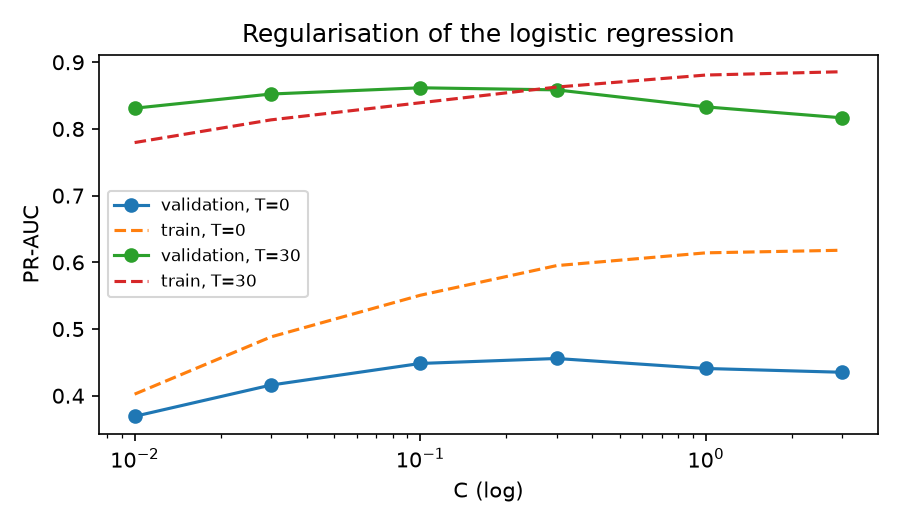
\includegraphics[width=0.6\linewidth]{logreg_C.png}
  \caption{Validation and train PR-AUC of the logistic regression as a function of $C$ (bias / variance).}
  \label{fig:C}
\end{figure}
\begin{figure}[p]
  \centering
  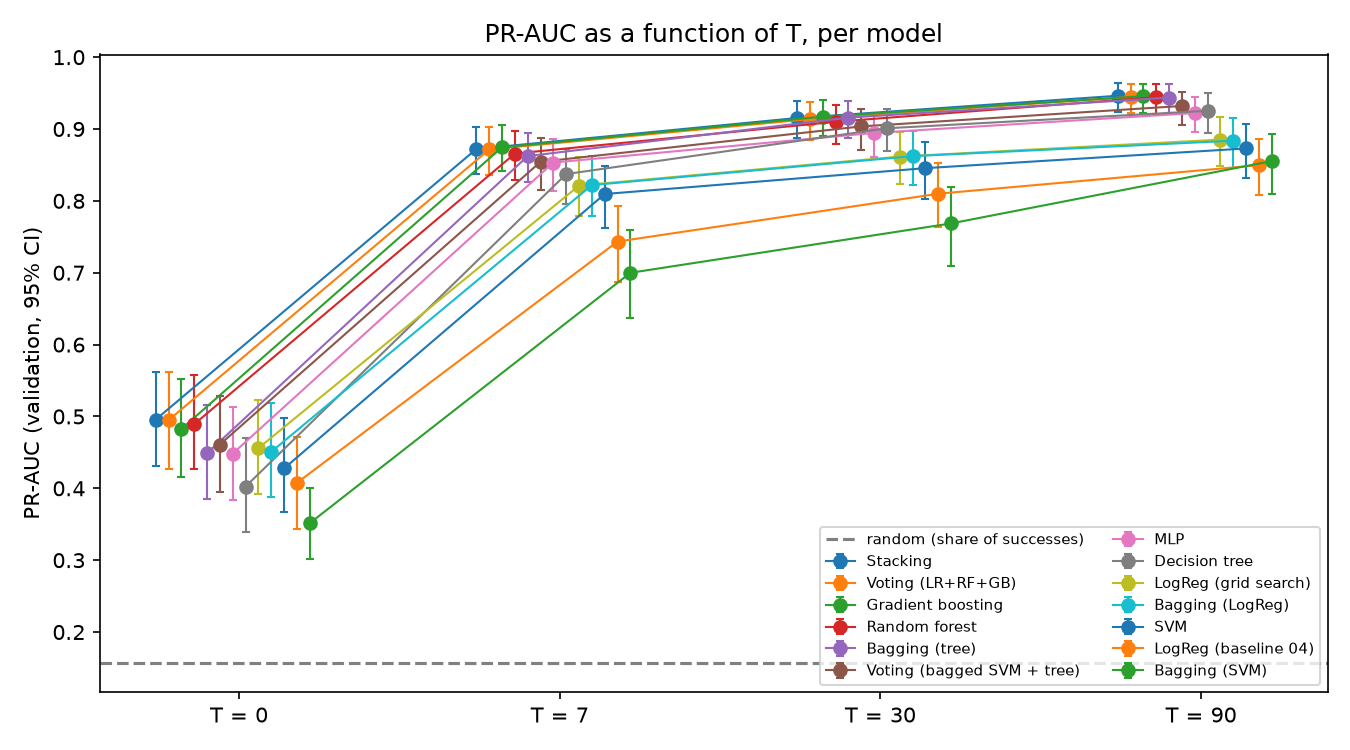
\includegraphics[width=0.85\linewidth]{prauc_vs_T_models.png}
  \caption{Validation PR-AUC as a function of $T$ for every model, with 95\% bootstrap confidence intervals.}
  \label{fig:prauc}
\end{figure}
\begin{figure}[p]
  \centering
  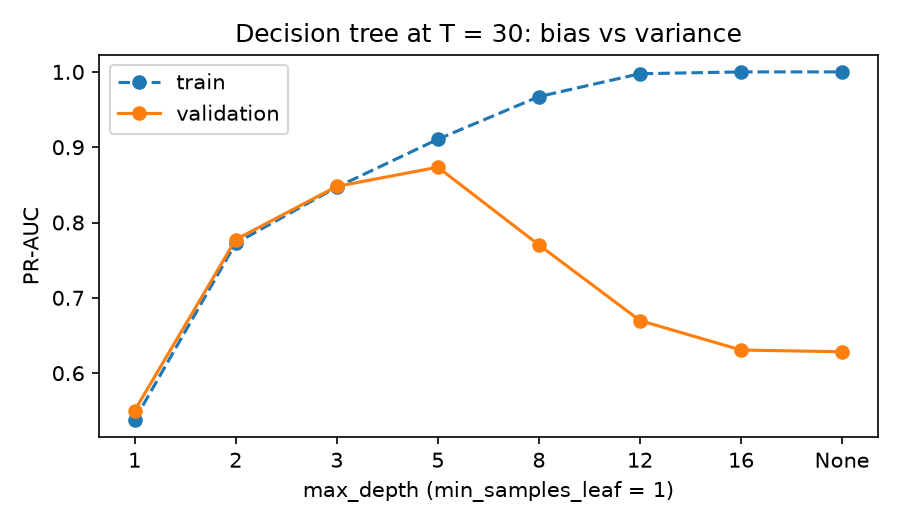
\includegraphics[width=0.6\linewidth]{tree_depth.png}
  \caption{Train and validation PR-AUC of a decision tree at $T = 30$ as a function of its depth
  (one game per leaf allowed): bias on the left, variance on the right.}
  \label{fig:tree}
\end{figure}
\begin{figure}[p]
  \centering
  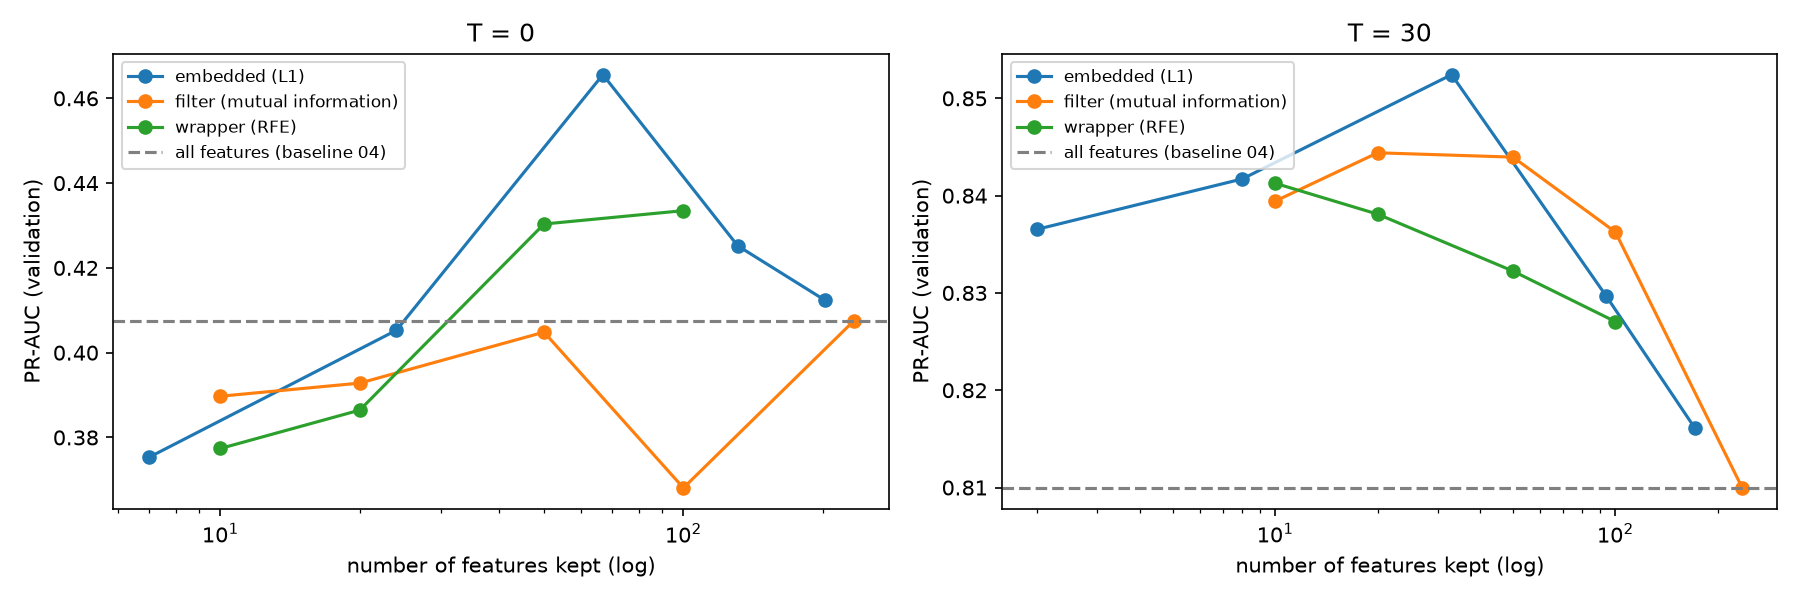
\includegraphics[width=0.9\linewidth]{feature_selection.png}
  \caption{Validation PR-AUC of the baseline logistic regression after feature selection, as a function of
  the number of features kept (notebook 06).}
  \label{fig:fs}
\end{figure}
\begin{figure}[p]
  \centering
  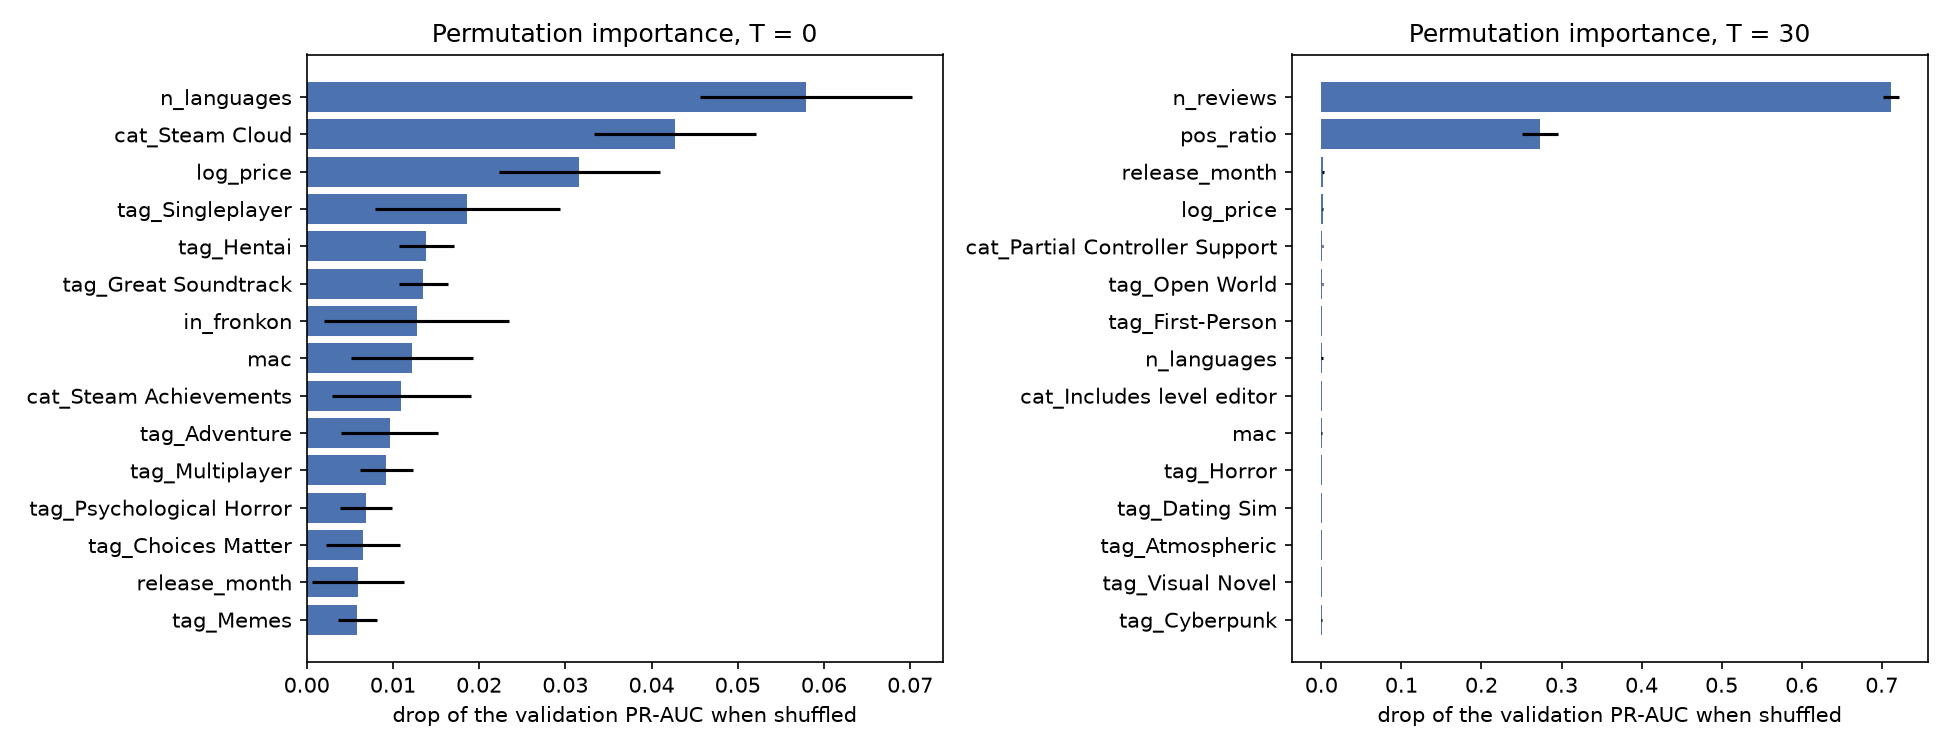
\includegraphics[width=0.9\linewidth]{permutation_importance.png}
  \caption{Permutation importance of a gradient boosting on the validation set: drop of the PR-AUC when a
  feature is shuffled (15 most important features, notebook 06).}
  \label{fig:perm}
\end{figure}

\end{document}
